\section{CKAN}
\label{sec:ckan-webapp}

As said in Chapter \ref{chp:rdf-builder}, the \ac{RDF} Graph Builder get the data from three different sources, and one of these sources is the CKAN Open Data Portal of the city (Comune di Sona in this case). The main idea is to use this open source portal in order to facilitate the publication of data on the web and be aligned with other Italian and foreign cities. At the same time, this portal provides the catalog  compliant with the \verb#DCAT-AP_IT# metadata profile, and this allows published data to be made available in regional, national and European portals as well. In addition, the presence of data in \acl{LOD} format does not preclude the use of the CKAN portal, despite the fact that the latter's data achieve a three-star rating according to Tim Berners-Lee's classification introduced in Section \ref{sec:lod-stars}. In fact, in addition to having a lower management cost \cite{bauer2011linked}, this portal allows the publication of data that in \acl{LOD} format would not be publishable, or for which an ontology describing them has not yet been developed. It also allows original resources to be reused for other tasks, either by the municipality or by companies or citizens.

\paragraph*{}
The entire project is available under an open source license on GitHub at the link \url{https://github.com/luca-martinelli-09/ckan}. The final result built for the Comune di Sona is shown in Figure \ref{fig:ckan-sona}. For ease of installation and deployment, moreover, the portal has been containerized to produce a Docker\footnote{\url{https://www.docker.com/}} image.

\begin{figure}[!ht]
  \centering
  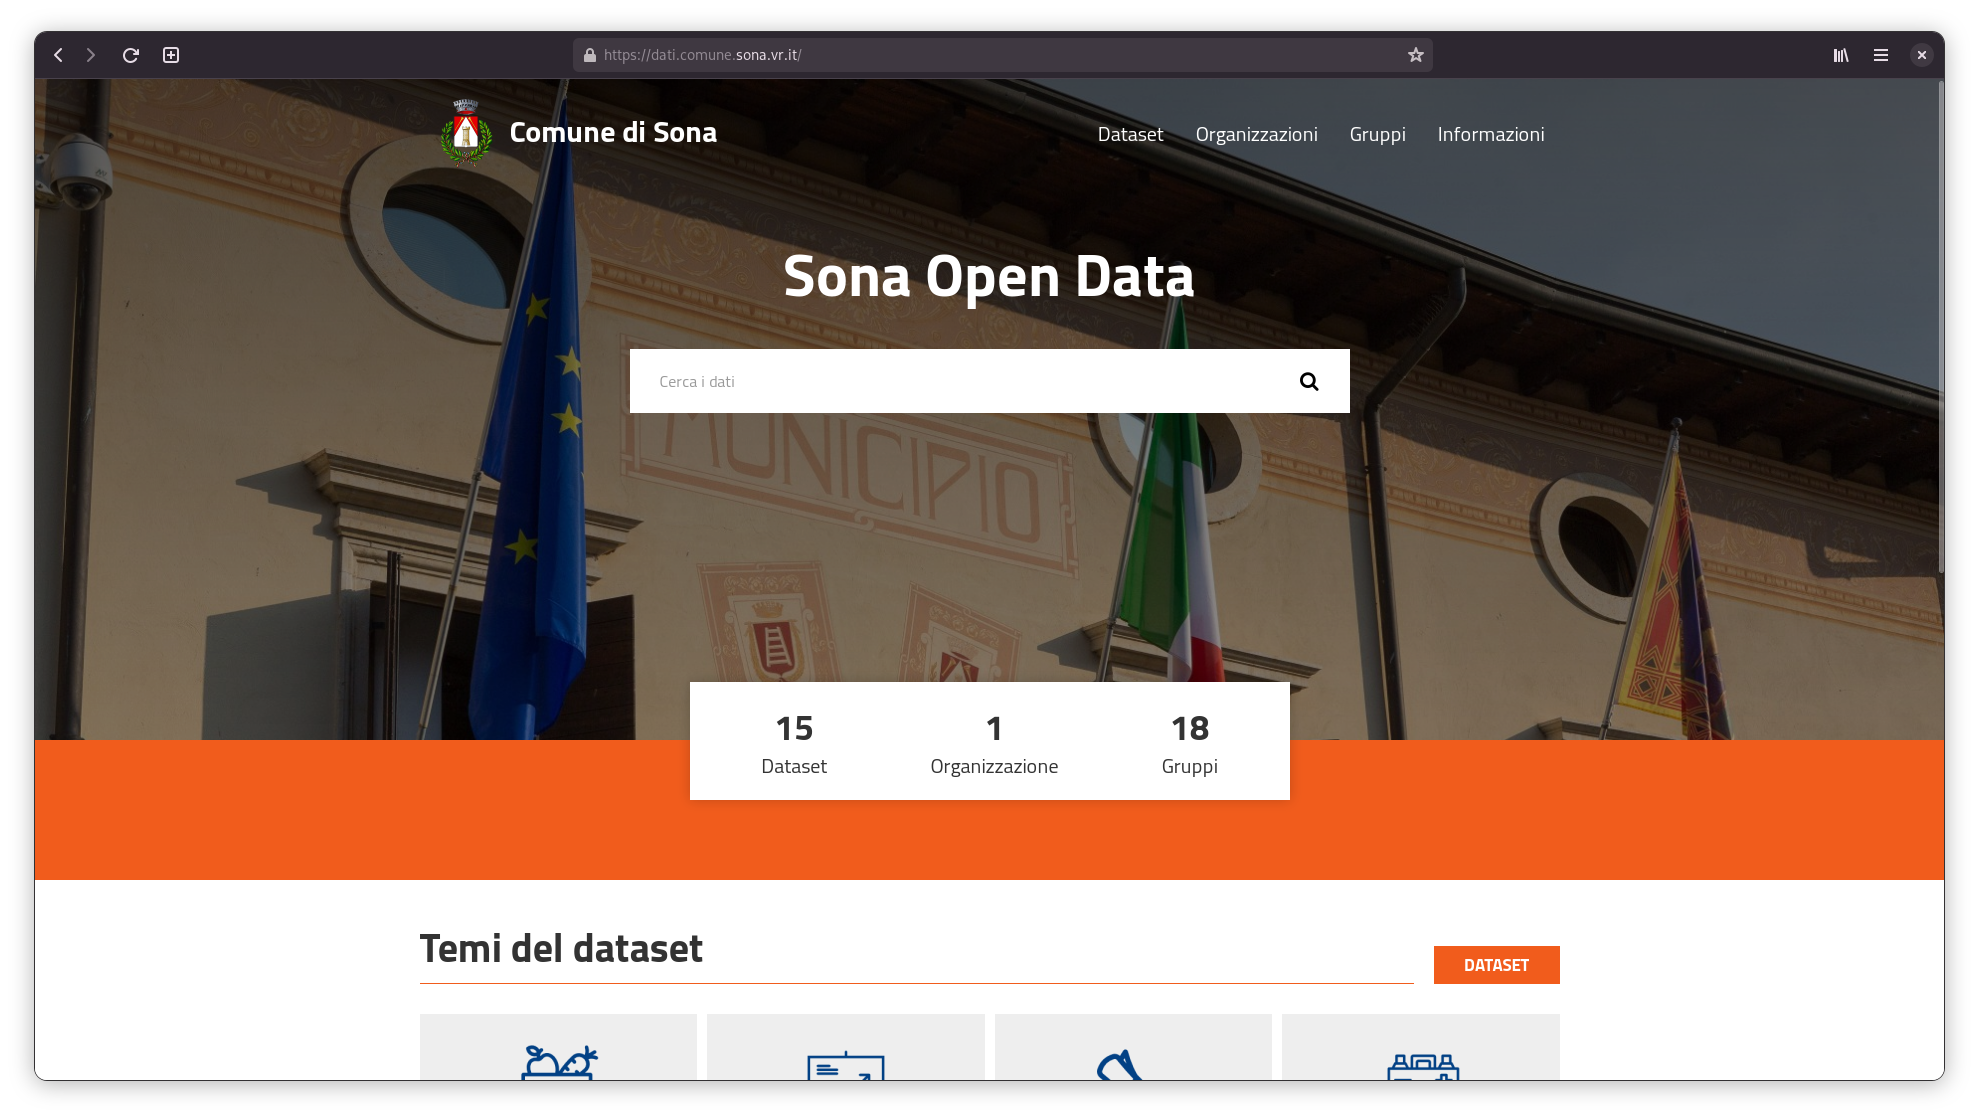
\includegraphics[width=\columnwidth]{images/ckan/ckan-sona}
  \caption{The CKAN Open Data portal for the Comune di Sona.}
  \label{fig:ckan-sona}
\end{figure}

\paragraph*{}
The Open Data portal extends the CKAN 2.9 Docker image provided by the Open Knowledge Foundation,\footnote{\url{https://github.com/okfn/docker-ckan}} installing the required plugins.